\documentclass[main.tex]{subfiles}
\begin{document}

Python 在 MacOS 和 Unix/Linux 操作系统是默认安装好的,
但版本一般是 \texttt{2.x},
且没有图形用户界面\index{图形用户界面, Graphic User Interface},
只适合在终端\index{终端, Terminal}命令行上进行交互运行或脚本运行。
微软视窗没有默认安装 Python。在 MacBook 在上选 Terminal,打开一个终端窗口,执行命令 python 后就见到\\

\begin{spacing}{0.9}
\noindent\texttt{\$python}\\

\noindent\texttt{WARNING: Python 2.7 is not recommended. }

\noindent\texttt{This version is included in macOS for compatibility with legacy software. }

\noindent\texttt{Future versions of macOS will not include Python 2.7. }

\noindent\texttt{Instead, it is recommended that you transition to using 'python3' from within}

\noindent\texttt{Terminal.}\\

\noindent\texttt{Python 2.7.18 (default, Oct  2 2021, 04:20:39) }

\noindent\texttt{[GCC Apple LLVM 13.0.0 (clang-1300.0.29.1) [+internal-os, }

\noindent\texttt{ptrauth-isa=deploymen on darwin}

\noindent\texttt{Type "help", "copyright", "credits" or "license" for more information.}

\noindent\texttt{>>>} \\
\end{spacing}
\noindent 输入 \texttt{exit()} 后按回车键退出。

本书采用 Python \texttt{3.x}。如果安装了 Python 3.x,则在命令行执行命令 
 “\texttt{python3}”  可开启交互运行模式。MacBook 上大约见到\\
 
\begin{spacing}{0.9}
	\noindent\texttt{\$python3}\\
	
	\noindent\texttt{Python 3.9.8 (main, Nov 10 2021, 03:55:42)  }
	
	\noindent\texttt{[Clang 13.0.0 (clang-1300.0.29.3)] on darwin}

	\noindent\texttt{Type "help", "copyright", "credits" or "license" for more information.}
	
	\noindent\texttt{>>>} \\
\end{spacing} 

\noindent 由命令  “\texttt{python3 file\_name}”  可以执行写在文件名
\texttt{file\_name} 中的 Python 3.x 代码。因为本书在集成开发环境(IDE - Integrated Development Environment)\index{集成开发环境, IDE}里操作,所以这里略去单纯的 Python 3.x 安装过程。

Python 有好几种免费的,且功能卓越的 IDE 软件。本书采用 Spyder,它提供一个优秀的开发平台和用户界面,进行 Python 的代码编辑、交互运行和图形绘制。Jupyter 也提供这样的开发平台,它以互联网浏览器为用户界面。其它很受欢迎并且为软件开发人员广泛使用的免费 IDE 有 Microsoft Visual Studio Code (https://code.visualstudio.com) 和 IntelliJ (Community 版本) (https://www.jetbrains.com)。
这两种 IDE 支持除了 Python 以外的其它语言,如 Java,JavaScript,Node.js 和 C++ 等。但 Python 以及它的一些常用包和库需要另行安装和配置,我们不在本书中使用。  


不管是在微软视窗还是苹果 MacBook 等上,若以简单起见,可访问

\,\,\,\,\texttt{https://www.spyder-ide.org} 

\noindent 而只安装 Spyder。

若想同时安装 Spyder 和 Jupyter, 则可选择 
安装 Anaconda Navigator。 网址是:

\,\,\,\,\texttt{https://www.anaconda.com} 。

\noindent 需要注意的是,个人版本(Individual Edition)是免费的,而其它版本则不是。个人版本从

\,\,\,\,\texttt{https://www.anaconda.com/products/individual} 

\noindent 下载安装。打开 Anaconda Navigator 后所见如图 \ref{fig:2.1.1},然后单击 Spyder 下面的 Launch 就会打开 Spyder。

\begin{figure}[h]
	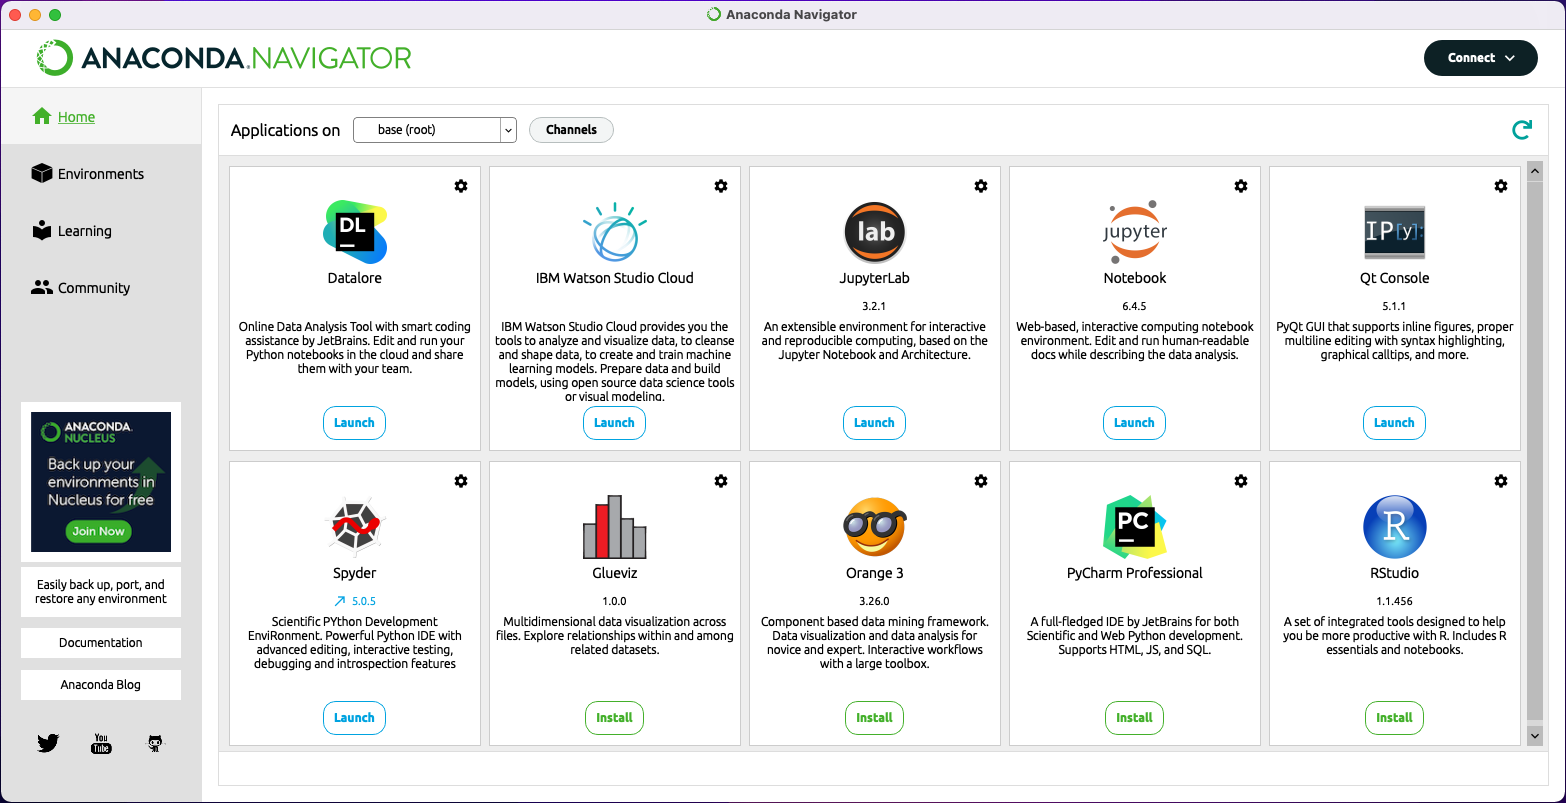
\includegraphics[width=1.0\textwidth]{png/anaconda_navig.png}
	\caption{Anaconda Navigator}\label{fig:2.1.1}
\end{figure}

\end{document} 
